\ifdefined\included
\else
\documentclass[a4paper,11pt,twoside]{StyleThese}
\usepackage{amsmath,amssymb}             % AMS Math
\usepackage[french]{babel}
\usepackage[utf8]{inputenc}
\usepackage[T1]{fontenc}
\usepackage{tabularx}
%\usepackage{tabular}
\usepackage{multirow}


\usepackage[tight,footnotesize]{subfigure}
\usepackage{algorithm} %To allow algorithm environment
\usepackage{algpseudocode} %Provides algorithmic environment

\usepackage{hhline}
\usepackage[left=1.5in,right=1.3in,top=1.1in,bottom=1.1in,includefoot,includehead,headheight=13.6pt]{geometry}
\renewcommand{\baselinestretch}{1.05}

% Table of contents for each chapter

\usepackage[nottoc, notlof, notlot]{tocbibind}
\usepackage[french]{minitoc}
\setcounter{minitocdepth}{2}
\mtcindent=15pt
% Use \minitoc where to put a table of contents

\usepackage{aecompl}

% Glossary / list of abbreviations

\usepackage[intoc]{nomencl}
\renewcommand{\nomname}{Liste des Abréviations}

\makenomenclature

% My pdf code

\usepackage{ifpdf}

\ifpdf
  \usepackage[pdftex]{graphicx}
  \DeclareGraphicsExtensions{.jpg}
  \usepackage[a4paper,pagebackref,hyperindex=true]{hyperref}
  \usepackage{tikz}
  \usetikzlibrary{arrows,shapes,calc}
\else
  \usepackage{graphicx}
  \DeclareGraphicsExtensions{.ps,.eps}
  \usepackage[a4paper,dvipdfm,pagebackref,hyperindex=true]{hyperref}
\fi

\graphicspath{{.}{images/}}

%nicer backref links
\renewcommand*{\backref}[1]{}
\renewcommand*{\backrefalt}[4]{%
\ifcase #1 %
(Non cité.)%
\or
(Cité en page~#2.)%
\else
(Cité en pages~#2.)%
\fi}
\renewcommand*{\backrefsep}{, }
\renewcommand*{\backreftwosep}{ et~}
\renewcommand*{\backreflastsep}{ et~}

% Links in pdf
\usepackage{color}
\definecolor{linkcol}{rgb}{0,0,0.4} 
\definecolor{citecol}{rgb}{0.5,0,0} 
\definecolor{linkcol}{rgb}{0,0,0} 
\definecolor{citecol}{rgb}{0,0,0}
% Change this to change the informations included in the pdf file

\hypersetup
{
bookmarksopen=true,
pdftitle="Évaluation de la sécurité des équipements grand public connectés à Internet",
pdfauthor="Yann BACHY", %auteur du document
pdfsubject="Thèse", %sujet du document
%pdftoolbar=false, %barre d'outils non visible
pdfmenubar=true, %barre de menu visible
pdfhighlight=/O, %effet d'un clic sur un lien hypertexte
colorlinks=true, %couleurs sur les liens hypertextes
pdfpagemode=None, %aucun mode de page
pdfpagelayout=SinglePage, %ouverture en simple page
pdffitwindow=true, %pages ouvertes entierement dans toute la fenetre
linkcolor=linkcol, %couleur des liens hypertextes internes
citecolor=citecol, %couleur des liens pour les citations
urlcolor=linkcol %couleur des liens pour les url
}

% definitions.
% -------------------

\setcounter{secnumdepth}{3}
\setcounter{tocdepth}{2}

% Some useful commands and shortcut for maths:  partial derivative and stuff

\newcommand{\pd}[2]{\frac{\partial #1}{\partial #2}}
\def\abs{\operatorname{abs}}
\def\argmax{\operatornamewithlimits{arg\,max}}
\def\argmin{\operatornamewithlimits{arg\,min}}
\def\diag{\operatorname{Diag}}
\newcommand{\eqRef}[1]{(\ref{#1})}

\usepackage{rotating}                    % Sideways of figures & tables
%\usepackage{bibunits}
%\usepackage[sectionbib]{chapterbib}          % Cross-reference package (Natural BiB)
%\usepackage{natbib}                  % Put References at the end of each chapter
                                         % Do not put 'sectionbib' option here.
                                         % Sectionbib option in 'natbib' will do.
\usepackage{fancyhdr}                    % Fancy Header and Footer

% \usepackage{txfonts}                     % Public Times New Roman text & math font
  
%%% Fancy Header %%%%%%%%%%%%%%%%%%%%%%%%%%%%%%%%%%%%%%%%%%%%%%%%%%%%%%%%%%%%%%%%%%
% Fancy Header Style Options

\pagestyle{fancy}                       % Sets fancy header and footer
\fancyfoot{}                            % Delete current footer settings

%\renewcommand{\chaptermark}[1]{         % Lower Case Chapter marker style
%  \markboth{\chaptername\ \thechapter.\ #1}}{}} %

%\renewcommand{\sectionmark}[1]{         % Lower case Section marker style
%  \markright{\thesection.\ #1}}         %

\fancyhead[LE,RO]{\bfseries\thepage}    % Page number (boldface) in left on even
% pages and right on odd pages
\fancyhead[RE]{\bfseries\nouppercase{\leftmark}}      % Chapter in the right on even pages
\fancyhead[LO]{\bfseries\nouppercase{\rightmark}}     % Section in the left on odd pages

\let\headruleORIG\headrule
\renewcommand{\headrule}{\color{black} \headruleORIG}
\renewcommand{\headrulewidth}{1.0pt}
\usepackage{colortbl}
\arrayrulecolor{black}

\fancypagestyle{plain}{
  \fancyhead{}
  \fancyfoot{}
  \renewcommand{\headrulewidth}{0pt}
}

%\usepackage{MyAlgorithm}
%\usepackage[noend]{MyAlgorithmic}
\usepackage[ED=MITT - STICIA, Ets=INP]{tlsflyleaf}
%%% Clear Header %%%%%%%%%%%%%%%%%%%%%%%%%%%%%%%%%%%%%%%%%%%%%%%%%%%%%%%%%%%%%%%%%%
% Clear Header Style on the Last Empty Odd pages
\makeatletter

\def\cleardoublepage{\clearpage\if@twoside \ifodd\c@page\else%
  \hbox{}%
  \thispagestyle{empty}%              % Empty header styles
  \newpage%
  \if@twocolumn\hbox{}\newpage\fi\fi\fi}

\makeatother
 
%%%%%%%%%%%%%%%%%%%%%%%%%%%%%%%%%%%%%%%%%%%%%%%%%%%%%%%%%%%%%%%%%%%%%%%%%%%%%%% 
% Prints your review date and 'Draft Version' (From Josullvn, CS, CMU)
\newcommand{\reviewtimetoday}[2]{\special{!userdict begin
    /bop-hook{gsave 20 710 translate 45 rotate 0.8 setgray
      /Times-Roman findfont 12 scalefont setfont 0 0   moveto (#1) show
      0 -12 moveto (#2) show grestore}def end}}
% You can turn on or off this option.
% \reviewtimetoday{\today}{Draft Version}
%%%%%%%%%%%%%%%%%%%%%%%%%%%%%%%%%%%%%%%%%%%%%%%%%%%%%%%%%%%%%%%%%%%%%%%%%%%%%%% 

\newenvironment{maxime}[1]
{
\vspace*{0cm}
\hfill
\begin{minipage}{0.5\textwidth}%
%\rule[0.5ex]{\textwidth}{0.1mm}\\%
\hrulefill $\:$ {\bf #1}\\
%\vspace*{-0.25cm}
\it 
}%
{%

\hrulefill
\vspace*{0.5cm}%
\end{minipage}
}

\let\minitocORIG\minitoc
\renewcommand{\minitoc}{\minitocORIG \vspace{1.5em}}

\usepackage{multirow}
%\usepackage{slashbox}

\newenvironment{bulletList}%
{ \begin{list}%
	{$\bullet$}%
	{\setlength{\labelwidth}{25pt}%
	 \setlength{\leftmargin}{30pt}%
	 \setlength{\itemsep}{\parsep}}}%
{ \end{list} }

\newtheorem{definition}{Définition}
\renewcommand{\epsilon}{\varepsilon}

% centered page environment

\newenvironment{vcenterpage}
{\newpage\vspace*{\fill}\thispagestyle{empty}\renewcommand{\headrulewidth}{0pt}}
{\vspace*{\fill}}

\usepackage{tablefootnote}
\sloppy
\begin{document}
\setcounter{chapter}{0} %% Numéro du chapitre précédent ;)
\dominitoc
\faketableofcontents
\fi

\chapter{Construction et Maintien de l'État du Monde}
\label{chapter1}
\minitoc


\section{Contexte}
\subsection{Défis à relever}
Le robot est un système pouvant percevoir, comprendre et agir sur son environnement. Comprendre son environnement suppose de pouvoir raisonner sur les données de perception afin d'en extraire des données de plus haut niveau d'abstraction, permettant d'avoir une estimation de la situation et ainsi de prendre les décisions adéquates pour accomplir la tâche qu'il lui incombe. C'est la célèbre boucle perception-action.

Avec le progrès récent de la robotique, les robots commencent à arriver dans les usines pour travailler aux côtés d'humains, ainsi que dans les foyers comme robot d'assistance. Adapter les capacités de raisonnements du robot à ce nouveau monde, qui est par définition modelé pour l'homme, représente un défi pour la recherche. Cet environnement humain est composé
d'éléments statiques tel que les murs, d'éléments pouvant évoluer au cours d'une interaction (déplacement, remplissage, activation...) que nous appellerons les objets, et enfin d'éléments pouvant se mouvoir, agir sur les objets, et interagir entre eux que nous appellerons les agents. Ces agents peuvent être robotiques ou humains.
Pour pouvoir agir dans un environnement humain, le robot doit donc pouvoir percevoir tous ces éléments énumérés précédemment et en extraire une représentation symbolique afin de décrire au mieux la situation et permettre à la couche décisionnelle d'agir de façon appropriée.


%TODO definir
%\section{Évaluation de la Situation}
%TODO
%définir... peut-être mettre dans la partie précédente?
\subsection{Évaluation de la situation}
La connaissance et la compréhension de la situation courante sont définies dans la littérature comme la connaissance de la situation (situation awarness). Le processus permettant d'acquérir et de maintenir la connaissance de la situation est appelé évaluation de la situation (situation assessment). Endsley explique dans \cite{endsley1995} que "la connaissance de la situation incorpore la compréhension d'un opérateur sur la situation globale, formant ainsi la base pour la prise de décision". La couche d'évaluation de la situation est donc fortement liée à la couche de prise de décision (aussi appelée supervision). Pour agir sur son environnement, le robot a besoin de décider quelle action entreprendre et quand agir. Pour prendre ce genre de décisions, la couche de supervision repose sur une couche inférieure pour fournir des informations à haut niveau d'abstraction sur l'environnement. Cela implique, pour la couche d'évaluation de la situation, de raisonner sur ce qui entoure le robot et d'extraire un ensemble de faits qui permet de modéliser une représentation symbolique de l'état du monde. Pour créer cette représentation symbolique, il est d'abord nécessaire au robot d'avoir une bonne estimation de l'état du monde et d'en avoir une représentation tridimensionnelle.



%With the recent advances in robotics, robots have begun to appear in our daily lives. The world of a robot is now populated with humans with whom it needs to interact. An important challenge for researchers is to adapt the robot's reasoning capabilities to this new world, which is by default shaped for humans. Human-robot interaction requires to equip the robot with explicit reasoning on the human and on its own capacities to achieve its tasks in a collaborative way with a human partner.

%In our concrete context, a robot and one or several human(s) share a physical environment, typically  a workshop or a domestic environment. The environment is composed of static walls and furnitures. What is dynamic is the fact that humans and robot move and manipulate objects.

%The role of SPARK (\textit{SPAtial Reasoning and Knowledge}) component described here in the robot control architecture is to permanently maintain a state of the world in order to provide a basis for the robot to plan, to act, to react and to interact. In addition, SPARK has been designed in order to take into account the following considerations.
%To tackle this challenge, robot's abilities must be enhanced.

%%%%%%%%%%%
\subsection{État de l'art}

De nombreux systèmes robotiques ont recours à un composant d'évaluation de la situation qui correspond aux besoins du robot dans une tâche applicative particulière. Dans \cite{beck2011}, le système d'évaluation de la situation est basé sur une chaîne de Markov dynamique pour modéliser les états de l'environnement et leur évolution. Les auteurs présentent une application pour un robot mobile navigant dans un passage étroit.
\cite{Kluge01situationassessment} présente une évaluation de la situation empirique pour robot mobile dans une zone à forte influence, permettant de reconnaître les situations d'obstruction volontaire.

Notre système permet non seulement d'effectuer l'agrégation des données de perception pour modéliser l'état du monde mais aussi le raisonnement géométrique. 
Nos travaux peuvent être comparés au "Grounded Situation Model" (GSM) introduit par Mavridis et Roy \cite{Mavridis2005} dans le sens où ils fournissent tout deux une représentation amodale du monde utilisée comme un médiateur entre les capteurs et le modèle symbolique. \cite{Coradeschi2013} présente une étude sur ces systèmes de fondement des symboles (symbol grounding) en robotique. \cite{Daoutis2009} \cite{Lemaignan2011}
présentent des exemples d'utilisation de ce genre de systèmes.

Les applications pour le raisonnement spatial \cite{OKeefe1999} sont multiples. Par exemple, cela a été utilisé pour le traitement du langage naturel pour des applications tel que la reconnaissance de direction \cite{Kollar10,Matuszek10}
ou le fondement du langage (language grounding) \cite{Tellex10}. \cite{Skubic2004} présente un raisonneur spatial intégré dans un robot qui calcule la position symbolique des objets.


% A variety of robotic systems have made a situation assessment component to fit the need of the robot in a particular task application. In \cite{beck2011}, the situation assessment system is based on Dynamic Markov chains to model the environment states and their evolution. It presents an application for a mobile robot to navigate in a narrow passage.
% \cite{Chella2010} aims to build a "higher order" perception, giving the robot the ability to reason on its own inner world.
% \cite{Kluge01situationassessment} presents an empirical assessment of situations for a mobile robot in a crowded public environment applied to recognize situations of deliberate obstruction. In our situation assessment software we focus on what is represented (human, objects ...) and we support heterogeneous type of sensors and data to provide a semantic interpretation of the environment with the aim to have a situation assessment capability that can be used in a various set of applications (see \ref{sec:applications}).


\section{Données capteurs}
\label{sec:collecte}
\subsection{Éléments statiques}
Un robot amené à interagir avec des humains est également amené à partager leur environnement. Que se soit dans un foyer ou une entreprise, cet environnement est composé de murs, d'escaliers de meubles... autant d'éléments statiques pouvant être des obstacles pour se mouvoir et manipuler les objets dans l'environnement. Ces éléments étant considérés comme "statiques", leur configuration peut être stockée dans la mémoire du robot (par exemple sous forme de carte 2D pour la navigation, comme dans la figure \ref{fig:map}) et directement utilisée par la couche d'exécution lorsque l'action à accomplir nécessite une navigation ou une manipulation, sans avoir à passer par la couche décisionnelle.

%MB put a map here to illustrate? Talk about gmapping?
\begin{figure}[ht!]
 \centering
  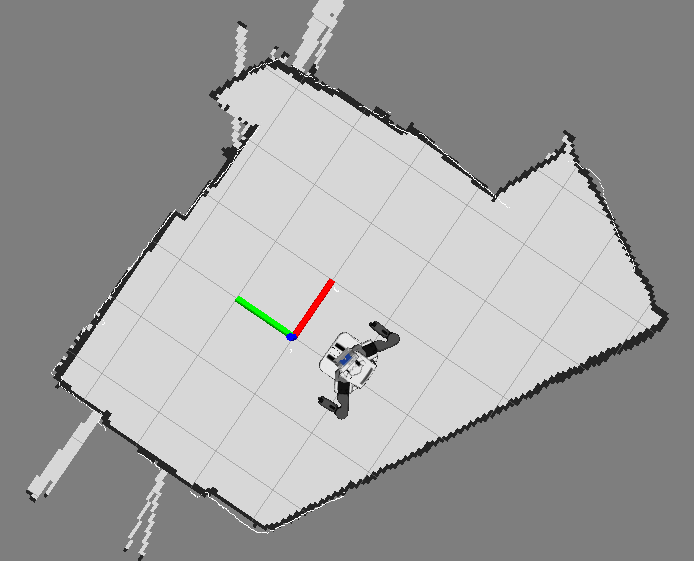
\includegraphics[width=0.59\linewidth]{./img/Map2d.png} 
  \caption {Exemple de carte pour la navigation et la localisation du robot}
  \label{fig:map}
\end{figure}

\subsection{Objets}
Les lieux de travail et de vie sont également composés d'objets divers. Des récipients, des outils, des vêtements, des appareils électroniques... autant d'éléments qui peuvent prendre des formes et fonctionnalités variées.
Certains de ces objets peuvent également avoir diverses états. Par exemple, une bouteille peut être vide ou pleine, un vêtement peut être propre ou sale, un appareil électronique peut être éteint ou allumé.
Ces objets sont pour la plupart manipulable au cours d'une interaction. Il est donc important que le robot puisse, afin d'agir correctement sur son environnement, reconnaître ces objets et dans la mesure du possible, connaître et suivre l'évolution de leur état.

Pour reconnaître les objets, diverses méthodes existent. Ces méthodes sont basées sur des solutions capteurs tel la stéréo vision \cite{murphy2005}
ou en utilisant un capteur RGBD tel la kinect \cite{tang2012}.
%TODO? ajouter illustration reconnaissance d'objets + image kinect
Ainsi, le robot est capable de détecter, reconnaître et positionner l'objet par rapport au reste de l'environnement.


\subsection{Proprioception et autres robots}
Pour comprendre la situation, le robot doit également pouvoir comprendre la situation des agents, à commencer par lui-même. Le robot est généralement composé de plusieurs membres, lui permettant de manipuler des objets, de changer son champ de vision ou de se déplacer. Il lui est donc nécessaire de connaître la configuration de ses propres membres. Cette faculté est appelée proprioception. Sur les robots, des capteurs de position permettent de transmettre la configuration des articulations, et ainsi de connaître la posture globale du robot. En utilisant les éléments statiques et à l'aide de techniques de localisation,
le robot peut également estimer sa position globale par rapport aux autres éléments de l'environnement.

\begin{figure}[ht!]
 \centering
  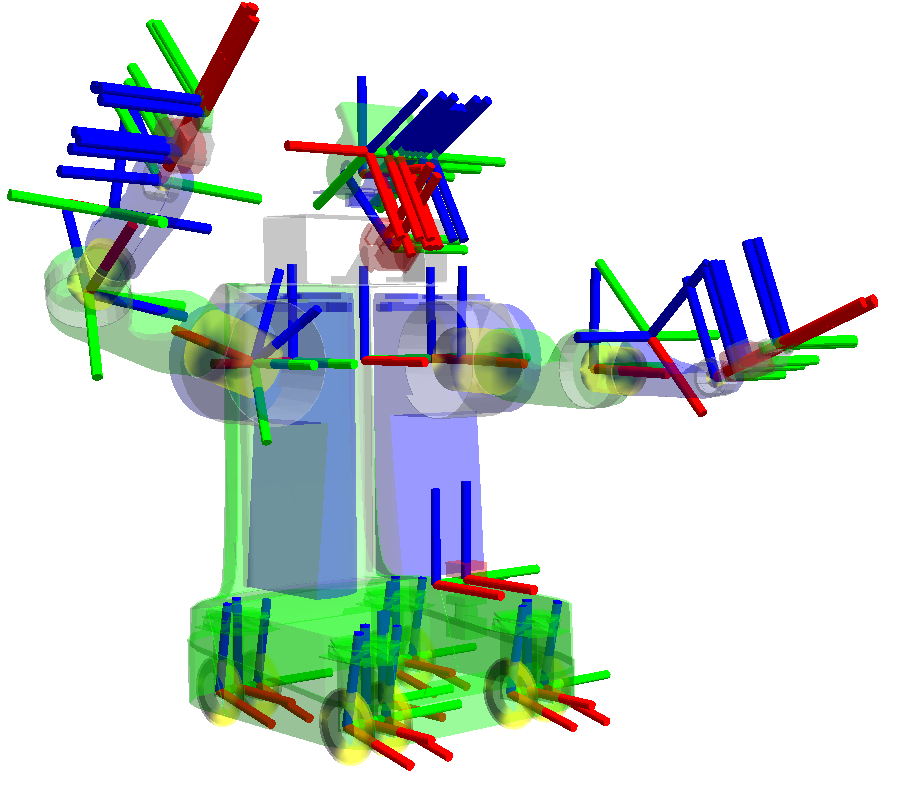
\includegraphics[width=0.59\linewidth]{./img/frames2.png} 
  \caption {Représentation tridimensionnelle du robot pr2 avec des repères pour chacune de ses articulations}
  \label{fig:frames}
\end{figure}

Dans le cas où l'interaction comporte plusieurs robots, il leur est possible de communiquer, à travers le réseau, leur configuration et ainsi permettre à chaque robot de pouvoir accéder directement à leurs propres données. Grâce à cela, il est possible à chaque système robotique de connaître la position et la configuration de chaque robot par rapport à l'environnement global.


\subsection{Humains}

Lorsqu'un ou plusieurs humains sont présents dans l'environnement, il est essentiel pour le robot de pouvoir au moins les détecter, voir de les reconnaître.
Tout comme le robot, l'homme possède plusieurs membres. Il est donc important de connaître la position de chaque homme mais aussi sa posture, et donc de percevoir la position de ses membres. Un capteur très utilisé pour détecter les humains est la kinect. Elle permet de connaître directement la position des différents membres de chaque humain. La figure \ref{fig:skeleton} présente la perception tridimensionnelle de la kinect et le suivi des membres de chaque humain ainsi que l'estimation de son squelette (de la position de ses membres) calculée à partir de cette perception.

%image kinect
\begin{figure}[ht!]
 \centering
  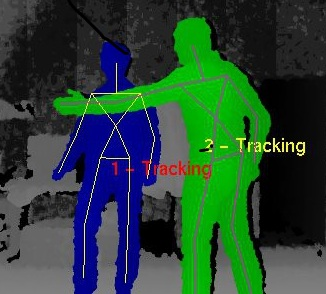
\includegraphics[width=0.59\linewidth]{./img/skeleton3.jpg} 
  \caption {Image provenant de la kinect et illustrant le suivi des humains et de leurs membres.}
  \label{fig:skeleton}
\end{figure}


De même, les équipements de capture de mouvements, tel que ceux utilisés dans le cinéma d'animation, peuvent permettre d'obtenir la position et la configuration des membres des humains. Cependant cette dernière solution nécessite aux humains de s'équiper de combinaison ayant des repères visuels pour les caméras de la capture de mouvements (voir figure \ref{fig:mocap}).

%image mocap
\begin{figure}[ht!]
 \centering
  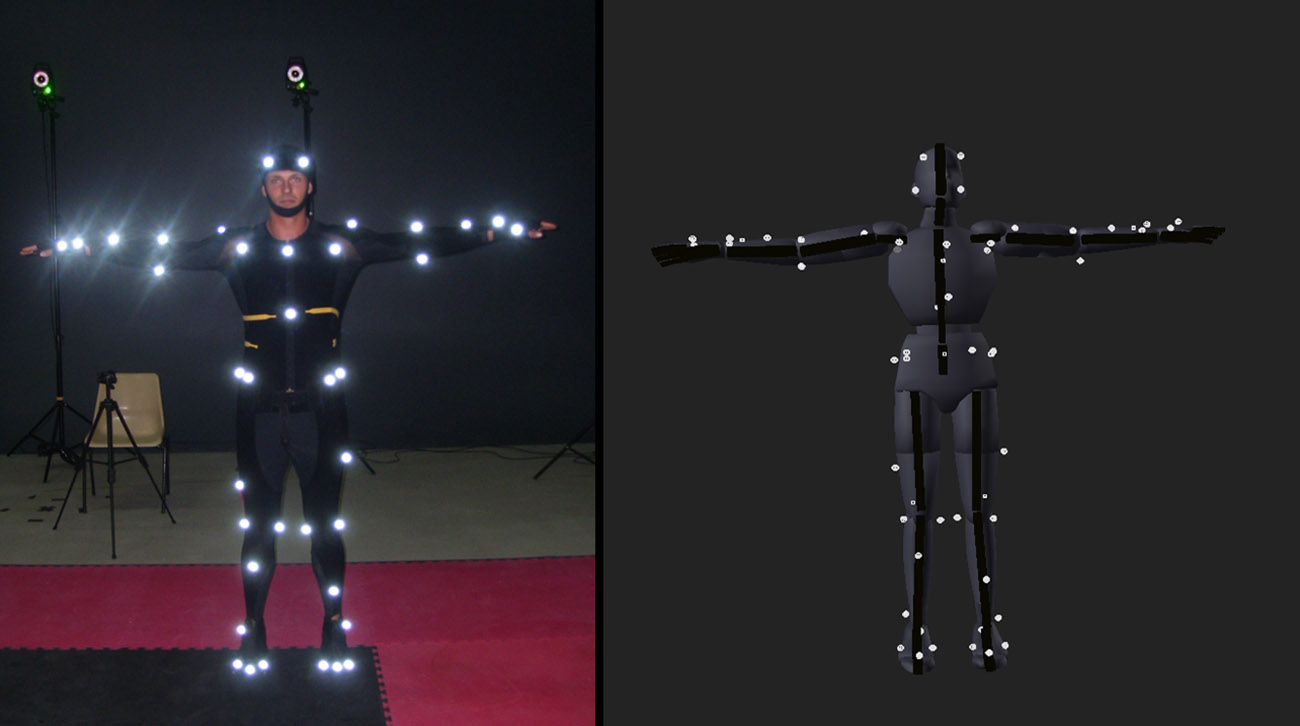
\includegraphics[width=0.69\linewidth]{./img/motionCap.jpg} 
  \caption {Exemple d'équipement de motion capture pour le suivi de l'homme et de sa posture. À gauche un homme équipé et à droite son modèle tridimensionnel.}
  \label{fig:mocap}
\end{figure}





\section{Calculs géométriques}
\label{sec:calculs}
\subsection{Modèle tridimensionnel et calculs de faits}
\label{sec:facts}

Une fois que le système robotique peut accéder aux données lui permettant d'obtenir la configuration de l'environnement et des divers éléments qui le composent, il est nécessaire, pour en extraire les informations pertinentes, de croiser les données. Pour ce faire, il faut dans un premier temps regrouper les données de position dans un repère commun afin que le robot puisse avoir une représentation globale de la scène. La figure \ref{fig:real} illustre cette unification avec une représentation en trois dimensions des divers éléments de l'environnement tel qu'ils sont perçus par le robot.

\begin{figure}[ht!]
 \centering
  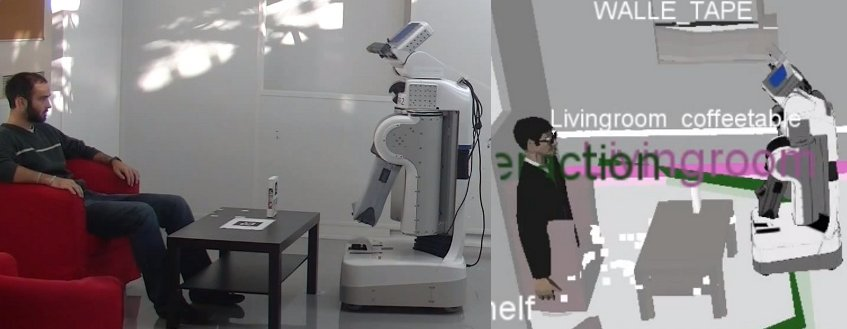
\includegraphics[width=0.99\linewidth]{./img/real.jpg} 
  \caption {Exemple d'environnement d'interaction homme robot (à gauche), et la représentation tridimensionnelle de cette même scène tel qu'elle est perçue par le robot (à droite)}
  \label{fig:real}
\end{figure}


L'unification des données capteur va permettre au système de maintenir un état du monde tridimensionnel comme dans la figure \ref{fig:real}. Pour améliorer le suivi de l'état du monde notamment au niveau des positions des divers éléments, il est parfois nécessaire d'établir un raisonnement basé sur des hypothèses, par exemple pour éviter de perdre la position d'un objet lorsqu'il n'est plus perçu. Ces raisonnements et hypothèses reposant sur des calculs géométriques et sur l'évaluation de la situation, ils seront présentés plus tard (en section \ref{sec:hypo}). 

La construction et le maintien du modèle tridimensionnel par agrégation des données provenant des divers capteurs va permettre de générer des liens symboliques entre les différents éléments de l'environnement. Dans notre système, nous représentons l'état du monde symbolique par une liste de \textit{faits}. Un \textit{fait} est traduit par une structure de données contenant divers champs que nous allons énumérés.

\begin{itemize}
\item \textit{Subject}: le sujet sur lequel la propriété s'applique. Il peut s'agir d'un agent (humain ou robotique), d'un objet ou du membre d'un agent (e.g.: \textit{Red\_Mug}, \textit{Human1}, \textit{PR2\_ROBOT}, \textit{Human1\_Right\_Hand}).
\item \textit{Property}: la propriété attachée au sujet du fait (\textit{Subject}) (e.g.: \textit{isOn}, \textit{isFull}, \textit{isMoving}, \textit{isPointing}, \textit{canSee}).
\item \textit{Target}: il se peut que la propriété relie l'entité-sujet \textit{Subject} avec une entité-cible \textit{Target}. Par exemple, si une entité \textit{RED\_BOOK} se trouve sur une entité \textit{KITCHEN\_TABLE}, \textit{RED\_BOOK} sera alors le sujet du fait tandis que \textit{KITCHEN\_TABLE} sera la cible.
\item \textit{PropertyType}: ce paramètre définit la catégorie dans laquelle on peut classer la propriété. Il peut s'agir par exemple d'une propriété de position, d'état, de mouvement, de posture ou d'accessibilité. En utilisant ce paramètre, lorsqu'un module extérieur ajoute un fait dont la propriété est inconnue, il reste possible de savoir quel type de propriété est décrite par ce fait. Cela permet également d'appliquer certains traitements aux faits en fonction de leur type.
\item \textit{Value}: selon la propriété, il est possible qu'une valeur y soit rattachée. Par exemple, la propriété décrivant l'état d'un container \textit{isFull} ou le déplacement d'une entité \textit{isMoving} peuvent prendre la valeur \textit{TRUE} ou \textit{FALSE}. Un autre exemple, si on représente la distance entre deux membres, comme la main (ou pince) du robot et la tête de l'homme, le paramètre \textit{Value} peut contenir la valeur \textit{DANGER}, \textit{CLOSE} ou \textit{FAR}. Dans certains cas, il est également possible de donner une valeur numérique à ce paramètre.
Dans d'autres cas, pour représenter le manque de connaissances sur une propriété et la "conscience" de ce manque, la valeur du fait peut aussi être \textit{unknown}.
\item \textit{Confidence}: ce chiffre entre 0 et 1 représente la fiabilité du fait. Cette valeur peut être liée à la fiabilité des capteurs ou résulter du calcul de la propriété.
\item \textit{Time}: ce paramètre permet d'enregistrer le moment auquel la propriété a été calculée.
\item \textit{FactObservability}: ce dernier paramètre représente la probabilité qu'un humain acquière la connaissance du fait s'il est capable de voir le sujet du fait. Plus de détails sur ce paramètres seront donnés dans le chapitre suivant.
\end{itemize}

Par exemple, le vecteur 
%TODO Make this as a table?
$<$ $Subject = Bob\_Right\_Hand$, $Property = isMovingToward$, $Target = HP\_Book$, $PropertyType = motion$, $Confidence = 0.8$, $time = 145571646570$, $FactObservability = 0.7$ $>$ représente le fait qu'à un temps \textit{time}, le bras droit de l'agent Bob (\textit{Bob\_Right\_Hand}) se dirige vers le livre "Harry Potter" (\textit{HP\_Book}).
Les sections suivantes décrivent les raisonnements géométriques et temporels 
permettant de générer ce genre de faits.


\subsection{Zones}
\label{sec:zones}

Pour avoir une première estimation de la situation, il est possible dans un premier temps de regarder l'emplacement des divers éléments. Pour ce faire, nous utilisons des zones ayant une signification sémantique particulière pour avoir une première catégorisation de la situation en fonction de la répartition des éléments par rapport à ces zones.

Nous définissons comme zone un emplacement délimité de l'environnement ayant une signification particulière. Ces zones peuvent être bidimensionnelles ou tridimensionnelles selon l'utilisation qui en est faite. Ces zones peuvent être statiques ou dynamiques et sont paramétrables. Les paramètres permettant de définir ces zones sont:
\begin{itemize}
\item le type de la zone: ce paramètre permet de catégoriser la zone. Ainsi une zone peut-être une pièce (comme une chambre, un salon...), une zone d'interaction avec un agent (par exemple en face de l'agent en question), une zone de danger...
Ce paramètre permet donc de donner un contexte sémantique à la zone concernée en l'associant à une catégorie.
\item le type d'éléments concernés par cette zone: une zone peut concerner que certains éléments de l'environnement. Ce paramètre permet de définir quel type d'éléments doivent être considérés. Il peut s'agir de toutes les entités (objets, et agents), ou simplement des agents ou d'un seul type d'entité (humain, robot ou objet). Les éléments ne faisant pas partie de la catégorie choisie seront ignorés des calculs effectués en lien avec cette zone.
\item le type de calcul lié à cette zone: ce paramètre permet de définir quels calculs doivent être fait. Ces calculs seront appliqués aux éléments concernés et se trouvant à l'intérieur de la zone.
\item le "propriétaire" de cette zone: une zone peut avoir un "propriétaire". Cela signifie que la zone sera "liée" à l'entité désignée comme propriétaire de la zone.  La position et l'orientation de la zone seront mis à jour avec la position et l'orientation de son propriétaire. Ainsi, il est possible de définir une zone d'interaction liée au robot par un trapèze positionné devant celui-ci. Si le robot bouge, la zone bougera avec lui pour toujours rester devant lui.
\end{itemize}

Pour reprendre l'exemple précédent, il est possible de définir une zone d'interaction devant le robot pour savoir si un humain se trouve dans cette zone et activer conditionnellement certains calculs, tel que l'orientation de l'humain pour savoir si celui-ci est dans une configuration permettant l'interaction.
La zone aura alors le vecteur de paramètres <\textit{interaction, humans, orientation, robot}>
Cette zone est illustrée par la figure \ref{fig:interaction} par une zone violette.
Dans l'exemple illustré, les faits (simplifiés ici) \textit{bob isInArea interaction} et \textit{bob isFacing pr2} sont générés. Le robot (\textit{pr2}) peut donc en déduire qu'il lui est directement possible de parler à \textit{bob} mais pas à \textit{greg} (il devra par exemple commencer par l'appeler).


\begin{figure}[ht!]
 \centering
  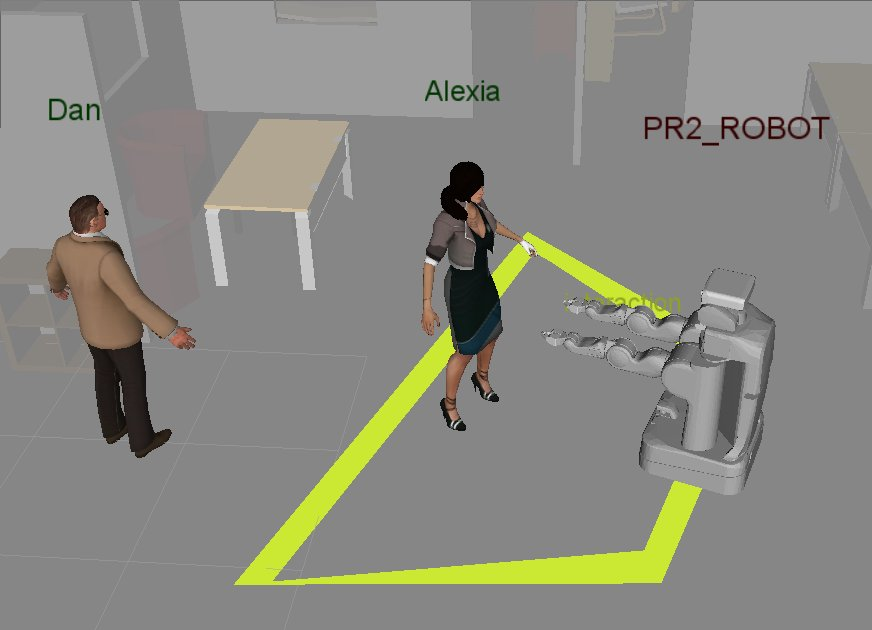
\includegraphics[width=0.69\linewidth]{./img/interactionarea.jpg} 
  \caption {Zone liée au robot Pr2 pour savoir si un humain est dans sa zone d'interaction. Ici bob se trouve dans la zone, le robot va donc calculer si celui-ci lui fait face}
  \label{fig:interaction}
\end{figure}

Ces zones peuvent être créées, mises à jour et supprimées pendant l'interaction (par exemple par le superviseur) et sont utiles pour avoir une première discrimination de la situation et des calculs conditionnels.


\subsection{Agencement}
\label{sec:agencement}
Pour pouvoir passer d'une représentation numérique à une représentation symbolique de l'environnement qui entoure le robot, il est nécessaire d'avoir, dans l'infrastructure logicielle du robot, un composant qui calcule les relations spatiales entre les objets. Ce composant fait une représentation tridimensionnelle de l'environnement en utilisant les données de position et d'orientation des différents éléments et leur mise à jour en temps réel pour tenir compte de l'état du monde courant. À partir de cette représentation 3d de l'état du monde, il calcule des propriétés d'agencement spatiale pour décrire la situation des objets.

Ce composant permet de calculer si un objet O1 se trouve au dessus d'un autre objet O2 (\textit{O1 isOn O2}), dans un objet O2 (\textit{O1 isIn O2}) ou à côté d'un objet O2 (\textit{O1 isNextTo O2}) comme illustré par la figure \ref{fig:spar}. Les détails de calculs et la méthode d'implémentation proviennent de travaux précédents et sont décrits dans \cite{sisbot2011situation}.


\begin{figure}[ht!]
 \centering
  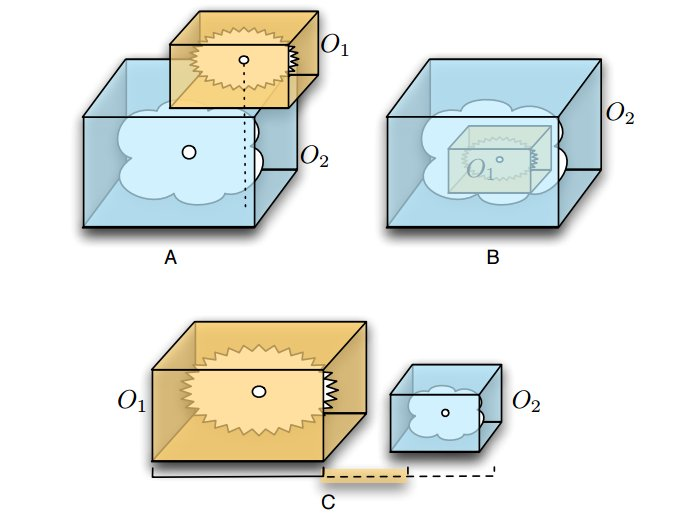
\includegraphics[width=0.5\linewidth]{./img/spar.jpg} 
  \caption {Relation spatiale entre deux objets: A) propriété \textit{isOn}, B) propriété \textit{isIn}, et C) propriété \textit{isNextTo}}
  \label{fig:spar}
\end{figure}


\subsection{Situation des agents}
\label{sec:situationAgents}

Quand le robot doit accomplir une tâche collaborative avec d'autres agents, et notamment avec des humains, il est primordial pour le système robotique d'identifier les activités humaines. Pour ce faire, nous utilisons un composant qui permet de surveiller chaque agent en utilisant des calculs de faits concernant les déplacements, la posture et la distance par rapport à certains points d'intérêt.

Le composant permettant de calculer ces faits enregistre en permanence les positions des entités, et ce pour une courte période de temps (quelques secondes). Afin de pouvoir stocker ces données temporairement et de les renouveler, nous avons créé une structure de données appelée buffer ciculaire temporel (time stamped circular buffer). La différence avec les buffers circulaires traditionnels est que les données y sont labellisées en fonction d'un marqueur temporel et qu'il est possible d'y accéder en utilisant le temps qui leur a été attribué. Ceci permet d'accéder à la donné de position des entités à un temps donné (moyennant de ne pas dépasser la taille du buffer).

Comme le suivi d'un agent peut s'avérer pertinent seulement dans certaines situations, le calcul des faits concernant n'importe quel agent peut être activé ou désactivé par requête. Ceci permet d'éviter de calculer en permanence des faits concernant tout les agents en ciblant seulement les agents qui se trouvent dans une situation nécessitant un suivi particulier.
Il est également possible de faire une requête pour activer le calcul de faits concernant un ou plusieurs des membres d'un agent. Lorsque le suivit d'un agent est activé, le composant calcul le déplacement de l'agent à partir des données présentes dans le buffer circulaire associé, afin de déterminer si l'agent est en train de se déplacer. En utilisant le buffer circulaire associé à l'agent et ceux associés aux autres entités, il est possible de calculer si l'agent se déplace en direction d'une entité en particulier (même si cette dernière est également en cours de déplacement) et l'évolution temporelle de la distance entre l'agent et un point d'intérêt. Ce calcul peut être aussi bien fait sur la position globale de l'agent ou sur l'un de ses membres (par exemple sur la main de l'homme).
En plus du mouvement, nous calculons également les distances entre les agents surveillés (respectivement les membres surveillés) et les autres entités.
De cette manière il est possible de savoir si un humain, ou l'un de ses membres, est proche d'un point d'intérêt (comme le robot ou un objet avec lequel il veut interagir).
Par exemple, ce module peut générer les faits (simplifiés ici) <\textit{HUMAN1 isMoving TRUE}> pour indiquer que l'humain \textit{HUMAN1} est en mouvement ou <\textit{HUMAN1\_RIGHT\_HAND isMovingToward BLUE\_BOOK}> pour indiquer que la main droite de l'humain se dirige en direction du livre bleu.

Le dernier type de fait concerne la posture de l'agent. En utilisant le buffer circulaire il est possible de savoir vers quoi l'humain pointait le doigt à un instant donné. Ceci peut être utile par exemple pour un module de fusion d'un système de dialogue. Ainsi, si un humain demande au robot "donne-moi ça", si la reconnaissance de parole est capable de fournir le temps pour lequel le mot "ça" a été prononcé, il est possible de faire une requête pour savoir quel objet était pointé par l'humain au moment où il a prononcé le mot "ça". Pour alléger la charge de calcul, ce fait est calculé seulement par requête (et non en permanence comme les autres). La requête renvoie une liste d'entités avec une probabilité pour chaque candidat potentiellement pointé.




\section{Hypothèses pour le maintien de l'état du monde}
\label{sec:hypo}
\subsection{Hypothèses de position}
%Put this in objects?


Dans leur quotidien, les humains sont occupés par divers activités (cuisine, nettoyage, bricolage...). Ces activités impliquent très souvent l'utilisation d'objets. Comme les robots sont fait pour assister les hommes dans leur tâches quotidiennes, il est crucial qu'ils puissent non seulement manipuler les objets, mais également suivre leur changement de position. Notre but ici n'est pas de discuter des différentes méthodes de suivi d'objet basé sur la perception mais d'expliquer comment le raisonnement sur les données de perception peut améliorer la détection et le suivi d'objet.

Localiser et suivre un objet n'est pas une tâche simple. En effet, l'objet peut être de petite taille et par conséquent être fréquemment occlus ou hors du champ visuel.
Les humains sont capables de connaître la localisation d'un objet même sans perception directe. Ils font en permanence des hypothèses sur la position des objets qu'ils ne peuvent pas voir et effectuent des raisonnement basés sur ces hypothèses. Pour travailler efficacement avec des humains, le robot doit être capable lui aussi de faire ce genre de raisonnements.

Pour ce faire, nous avons ajouté au composant qui maintient l'état du monde à jour la possibilité d'émettre des hypothèses de position lorsqu'un objet n'est pas visible.

Comme hypothèse de base, lorsque le robot est dans l'incapacité de voir l'objet (l'objet est hors du champs de vision ou est occlut), le système suppose que l'objet est à la même place et a la même orientation que la dernière fois qu'il l'a perçu. Dans la figure \ref{fig:occluded} 
le livre bleu n'est pas visible par le robot (car il est caché par la boîte rose). Cela signifie que le capteur de vision n'est plus capable de fournir la donnée de position de cet objet. Cependant, le système de maintient de l'état du monde le conserve tel quel dans le modèle de l'environnement car il sait que l'objet est occlut, et qu'il est donc normal qu'il ne soit pas détecté. Cette hypothèse de maintien de position est utilisée comme hypothèse par défaut. Cela signifie que s'il y a une autre hypothèse concernant la position d'un objet, nous choisirons cette dernière plutôt que celle par défaut.

\begin{figure}[ht!]
 \centering
  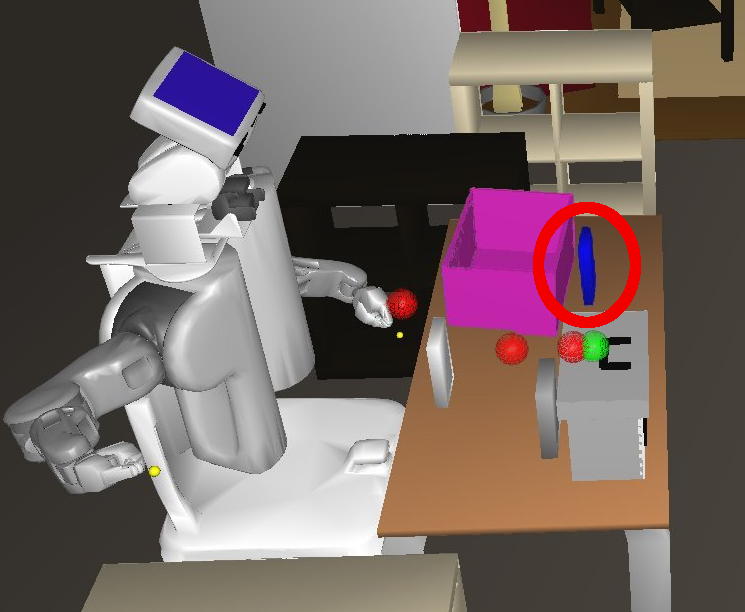
\includegraphics[width=0.69\linewidth]{./img/occluded.png} 
  \caption {Exemple d'État du monde où le système maintient les objets en position même s'ils ne sont pas directement perçus (comme le livre bleu).}
  \label{fig:occluded}
\end{figure}

Les autres hypothèses de position sont générées à partir des actions du robot et de l'homme. Si le robot attrape un objet, l'objet sera probablement caché par sa propre main, mais nous savons où l'objet se trouve (dans la main du robot).
Nous avons le même type d'hypothèse pour l'humain, en utilisant les observations sur la situation de l'humain (proximité avec un objet, posture, mouvement) présentées à la section \ref{sec:situationAgents}, il est possible de suivre les actions de l'homme, et ainsi de savoir quand un humain prend un objet ou le dépose.

En dernier lieu, nous avons également une hypothèse permettant de connaître la position des objets lorsque ceux-ci sont contenus dans d'autres objets.
Si un agent laisse tomber un objet dans un autre, même si il n'est pas possible de voir l'objet lâché, il est possible d'approximer sa position (par exemple en le mettant au centre du contenant).

\begin{figure}[ht!]
 \centering
  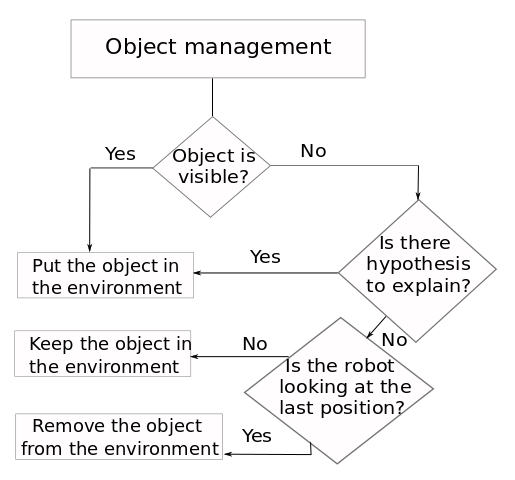
\includegraphics[width=0.70\linewidth]{./img/hypothesis.png} 
  \caption {Schéma de raisonnement pour gérer la position d'un objet. Les hypothèses sur la position des objets peuvent provenir d'une occlusion, d'un objet dans un conteneur ou dans la main d'un agent.}
  \label{obj_manag_fg}
\end{figure}

Pour résumé, le robot utilise en premier lieu la perception, puis s'il n'est pas possible de percevoir l'objet il utilise des hypothèses de position.
Si aucun des deux n'est disponible, il utilise la dernière position de l'objet, comme indiqué par la figure \ref{obj_manag_fg}.
Les hypothèses de position doivent être gérées en temps réel pour maintenir un modèle du monde cohérent.
Dans le cas où un objet a une hypothèse de position et est perçu en même temps, la position perçue est comparée avec celle donnée par l'hypothèse de position. Si la  position indiquée est incompatible (distance trop importante) l'hypothèse est alors supprimée car elle est considérée comme impossible.
Si un objet devrait pouvoir être perçu et ne l'est pas, alors l'hypothèse par défaut est annulée et la position de l'objet prend alors la valeur "unknown" pour indiquer que le robot ne sait pas où se trouve l'objet en question.

Ces hypothèses concernant la position des objets liés à un raisonnement top-down (symbolique vers sub-symbolique) permettent au robot d'avoir un suivi plus efficace des objets, spécialement quand ils sont occlus ou non perçus.


\subsection{Généralisation}


%TODO: généralisation du maintient du monde par la gestion des hypothèses (rempli / vide, chaud/froid...)
% Différent car ne modifi pas l'état du monde sub symbolique

Pour aller plus loin, nous travaillons actuellement à généraliser ces hypothèses. En effet, il est important de pouvoir suivre la position des objets, et donc d'établir des hypothèses pour pallier le manque de visibilité et avoir un suivi efficace de la position des objets, mais il est également important de connaître l'état des divers propriétés liées aux objets. Contrairement aux hypothèses de position, ces hypothèses n'influencent pas la représentation tridimensionnelle de la scène mais uniquement les données symboliques.

Ce maintien des hypothèses concernant l'état symbolique du monde est réalisé grâce à un module de reconnaissance d'actions appelé AIR (Action and Intention Recognizer), dont le fonctionnement est présenté au chapitre \ref{chapter4}.
Ce module transmet au module de gestion d'hypothèses (Hypotheses Manager) les actions détectées par le système.
Basé sur un nombre de règles liées aux actions, le module de gestion d'hypothèses est capable de mettre à jour certaines propriétés liées à l'état symbolique du monde.

Par exemple, si le module AIR détecte qu'un humain a versé le contenu \textit{C} d'un récipient \textit{B} (comme une bouteille) dans un autre récipient \textit{V} (comme un verre), le rôle du module de gestion des hypothèses sera d'envoyer une requête à la base de données pour mettre à jour l'état des propriétés liées à \textit{V} et \textit{B}. Ainsi, la propriété \textit{isEmpty} sera mise à faux pour \textit{V} et la propriété \textit{hasLiquid} sera ajoutée avec \textit{C} comme valeur (\textit{C} peut être par exemple de l'eau. Le module de gestion d'hypothèses sera également chargé de décrémenter la quantité de \textit{C} contenue dans \textit{B}.
Pour résumer, ce module de gestion d'hypothèses permet d'appliquer les effets (ou postconditions) liés à une action lorsque celle-ci est détectée. Il sera également en charge d'assurer la cohérence globale de l'état du monde.


Le schéma \ref{fig:hypo} présente l'architecture prévisionnelle permettant cette gestion d'hypothèses. Le module de gestion d'hypothèses peut envoyer des requêtes au module d'agrégation de données et de maintien du monde (Perceived Data Gathering) pour modifier la position d'un objet, ou à la base de données temporelle (présentée à la section suivante) pour modifier certains faits, et donc l'état du monde symbolique.

\begin{figure}[ht!]
 \centering
  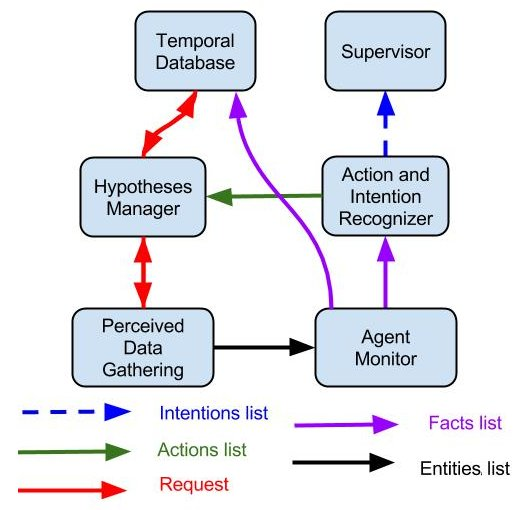
\includegraphics[width=0.7\linewidth]{./img/hypotheses_manager.jpg} 
  \caption {Schéma de l'architecture prévisionnelle pour le module de gestion des hypothèses.}
  \label{fig:hypo}
\end{figure}


%TODO: Temporal database here?
\section{Base de données temporelle}
\label{sec:db}
%%%%%%%%%%%%%%%%%%%%%%%%%%%%%%%%%%%%%%%%%%%%%%%%%%%%%%%%%%%%%%%%%%%
Nous avons présenté précédemment comment divers composants contribuent à maintenir un état du monde géométrique (sub-symbolique). Nous avons également présenté comment d'autres composants, à partir de l'état du monde géométrique et de raisonnements et calculs sur celui-ci, générant une liste de faits permettant une représentation symbolique de l'état du monde et une estimation de la situation.

Afin de regrouper ces données symboliques et permettre un accès standardisé et efficace, nous avons ajouté une base de données SQL à notre système.

\subsection{Gestion des données}
\label{sec:dbd}
La base de données peut gérer deux types de données: les données statiques et dynamiques. En effet, il est possible de connaître à priori certaines informations sur l'environnement tel que la couleur, le nom de certains objets ou leur type ou leur propriétaire. 
Nous avons donc dans notre base de données une première table permettant d'avoir des informations sur les diverses entités de l'environnement. Cette table peut être complétée en ligne si le système reçoit des informations complémentaires durant l'interaction (si le robot découvre de nouvelles propriétés statiques ou de nouveaux objets, que se soit par la perception ou le dialogue).

Concernant les données symboliques et notamment les \textit{faits} générés par les divers composants d'évaluation de la situation, la base de données récupère en permanence la liste de faits générée et publiée par chacun des modules. Cela permet de vérifier les changements apparus dans l'environnement pour mettre à jour la table de représentation symbolique de l'état du monde tel qu'il est perçu par le robot (\textit{ROBOT\_WS\_TBL} pour Robot World State Table).
Cette table est composée de faits qui sont considérés comme vrais et mis à jour en temps réel. Ces faits proviennent des divers modules d'évaluation de la situation et ont comme valeur temporelle la date où le fait a été détecté.

%blabla etat du monde + données statiques

\subsection{Gestion de la temporalité}
\label{sec:dbt}
L'une des valeurs ajoutées de cette base de données est l'aspect temporel.
En effet, lors d'une interaction homme robot, de nombreux événements peuvent se succéder et pour pouvoir comprendre et interpréter les actions et les élocutions de l'homme, il est important de considérer l'historique de l'interaction.

Nous avons donc ajouté une gestion de l'aspect temporel.
Pour ce faire, lorsqu'un fait est considéré comme vrai à partir d'un temps t1 et donc présent dans la table de représentation symbolique de l'état du monde perçu par le robot, le temps t1 lui est attribué jusqu'à ce que ce fait soit considéré comme faux à un temps t2.

Lorsque le fait est considéré comme faux en t2, ou lorsqu'il change de valeur, il est retiré de la table \textit{ROBOT\_WS\_TBL} pour être mis dans une table mémoire \textit{ROBOT\_MEM\_TBL}. Cette table contient également une liste de faits. À la différence de la table \textit{ROBOT\_WS\_TBL}, les faits de cette table peuvent être en double (deux faits identiques peuvent être présent dans la table si ils ont des temps différents) et représentent des faits passés. Pour ce qui est du temps associé, chaque fait a deux dates: la date t1 à laquelle le fait a commencé a être vrai (ou plutôt détecté comme étant vrai) et la date t2 à laquelle le fait a cessé d'être vrai (détecté comme étant faux).
Pour avoir un accès direct aux transitions, nous avons également ajouté une table d'événements \textit{EVENT\_TBL}. Lorsqu'une transition de fait est détectée (un fait n'est plus vrai ou change de valeur), en plus de le retirer de la table de faits courant et de l'ajouter à la table mémoire, nous ajoutons la transition avec la date de t2. 

Pour illustrer, nous prenons l'exemple où un homme \textit{H} prends un objet \textit{O} sur une table \textit{T} à un moment t2. Trois opérations seront faites dans la base de données:

\begin{itemize}
\item Le fait \textit{O isOn T} sera déplacé de la table \textit{ROBOT\_WS\_TBL} vers la table \textit{ROBOT\_MEM\_TBL}, avec t2 comme temps de fin.
\item Le fait  \textit{H hasInHand O} sera ajouté à la table \textit{ROBOT\_WS\_TBL} avec un temps t2.
\item L'événement \textit{H picks O} sera ajouté à la table \textit{EVENT\_TBL}.
\end{itemize}

Cette gestion du temps, des événements et de la mémoire permet de pouvoir réaliser des raisonnements temporels complexes sur les données symboliques et les liens temporels entre les différents faits. L'une des améliorations à venir est de permettre "d'oublier" les événements en fonction de leur date et de leur ancienneté pour éviter de saturer la mémoire dans le cas d'une utilisation longue durée.



% %TODO: improve clearness
% Another capacity of the database component is the event based time management. This provides memory to the system.
% When facts are received, the time of detection is present in one of their variables (as mentioned in \ref{sec:facts}). When the database manager detects a shift in a property, it updates the belief tables as explained in previous section, but it also records the event. To do so, we add a table filled with each event that occurs, recording the time when the property changes. As an example, if a Mug was on a table and the robot detects that the Mug is now in Bob's hand, it will remove the fact $<$\textit{Mug isOn $Kithen\_Table$}$>$ from the belief tables of agents able to perceive the change, and add the event $<$\textit{Bob pickUp Mug}$>$ in the event table.
% In addition to the event table, we add a memory table for each agent. This memory table stores facts that the agent has believed to be true. We use as starting time the time when the agent noticed a property, and as ending time the moment when the agent detects a change in it.
% One of the application can be to 
% %find correct terminology: reference finding? grounding? desambiguate?
% %Miki: This is quite nice actually. What about making real experiments on that? XD
% %Greg: Yep, we should! I put it in the conclusion
% %But we also have to work on robustifying the thing...
% understand when a human asks "Where is the mug that was on the table" by detecting in his memory table which mug she/he is talking about and looking in the current fact table where it currently is. In addition, the robot could even tell the related event that created the change: "It is now in the sink, Bob picked it up 5 minutes ago".



%%%%%%%%%%%%%%%%%%%%%%%%%%%%%%%%%%%%%%%%%%%%%%%%%%%%%%%%%%%%
\section{Implémentation}

Les composants décrits précédemment ont été implémentés dans une infrastructure logicielle open-source appelée TOASTER\footnote{TOASTER est disponible sur github à l'adresse https://github.com/Greg8978/toaster} (Tracking Of Agents and Spatio-TEmporal Reasonning).

L'un des avantages de TOASTER repose sur sa généricité et son adaptabilité grâce à une conception modulaire qui permet également d'étendre facilement l'infrastructure. En effet, comme présenté en section \ref{sec:collecte}, les données d'environnement peuvent parvenir de divers capteurs.

\subsection{Collecte de données et généricité}
\label{sec:PDG}
Pour que l'infrastructure logicielle soit utilisable avec n'importe quelle configuration de capteurs, un premier module permet de collecter toutes les données et de les mettre au format TOASTER. Tous les autres modules utiliseront ensuite l'état du monde au format exporté par ce module. Ce module chargé de collecter les données des divers capteurs est appelé \textit{PDG} pour Perceived Data Gathering.
Il permet à l'heure actuelle de gérer quatre types d'entrées pour l'homme, deux pour les objets, deux modèles de robot. Il gère également deux types de messages d'entrée: le ROS\footnote{http://www.ros.org/} et le pocolibs\footnote{https://www.openrobots.org/wiki/pocolibs}.

Un autre avantage de ce module est également sa simplicité d'extension. Ainsi, grâce au système d'héritage du C++ il est possible d'ajouter une entrée capteur pour détecter des objets, pour suivre l'homme ou un modèle de robot en seulement 50 à 200 lignes de code C++ (estimation basée sur les entrées déjà existantes).
Au démarrage du module ou à tout moment de l'interaction, il est possible de (re)configurer se module pour modifier les entrées à prendre en compte.

Durant la phase de développement de nouvelles fonctionnalités il est coûteux d'un point de vue matériel tout comme d'un point de vue temporel de faire des tests dans le monde réel. Pour permettre de tester rapidement et sans monopoliser de plateforme robotique, le module \textit{PDG} peut prendre en entrée des données de simulateur robotique tel que Gazebo\footnote{http://wiki.ros.org/gazebo} pour la configuration du robot, MORSE\cite{echeverria11} pour la configuration de l'homme, du robot et la vision des objets. En plus de ces simulateurs, un module intégré à TOASTER pour créer et tester des environnements d'interaction homme robot appelé \textit{toaster\_simu} a été créé. \textit{PDG} permet également d'avoir une configuration hybride.
Par exemple, il est possible d'utiliser les capteurs d'un robot réel ainsi que la détection d'objets dans le monde réel et de simuler le déplacement d'un humain (avec l'interface clavier).
Le module \textit{PDG} permet donc une grande flexibilité dans la configuration des données d'entrées. En exportant l'état du monde dans un format unique et invariable, \textit{PDG} permet aux autres modules TOASTER de s'abstraire de cette diversité et de conserver les mêmes formes de raisonnement, indépendamment de la configuration des capteurs et des données d'entrées de TOASTER.

\subsection{Outils de développement}
Pour aider au développement de nouvelles fonctionnalités et à la configuration de scénarios, un module de visualisation a été ajouté à l'infrastructure TOASTER. Ce module utilise le rviz\footnote{http://wiki.ros.org/rviz} pour afficher les différents éléments en trois dimensions, ce qui permet de comprendre la situation en affichant l'état du monde. Chaque entité est associée à un modèle 3D qui est positionné dans un environnement virtuel à la position et à l'orientation données par le module PDG. Le module affiche également les noms de chaque entité au dessus de leur modèle 3D. 
Le module permet également d'afficher les différentes zones présentes dans le module de gestion de zone (\textit{area\_manager}) avec leurs noms, comme présentée sur la figure \ref{fig:interaction}.
Concernant les faits exportés par le module de suivi d'agents (\textit{agent\_monitoring}), afin d'éviter la surcharge de l'interface, le fait \textit{isMoving} rend l'affichage du nom de l'agent plus intense selon si le système considère qu'il bouge. La donnée numérique de sa vitesse associée à ce fait permet également de faire varier cette intensité. Pour le fait \textit{isMovingToward}, une flèche reliant l'agent à l'entité vers laquelle il se déplace est tracée. L'intensité de la couleur de cette flèche varie également en fonction de l'indice de confiance du fait associé. Ce retour visuel est illustré par un exemple à la figure \ref{fig:moving}

\begin{figure}[ht!]
 \centering
  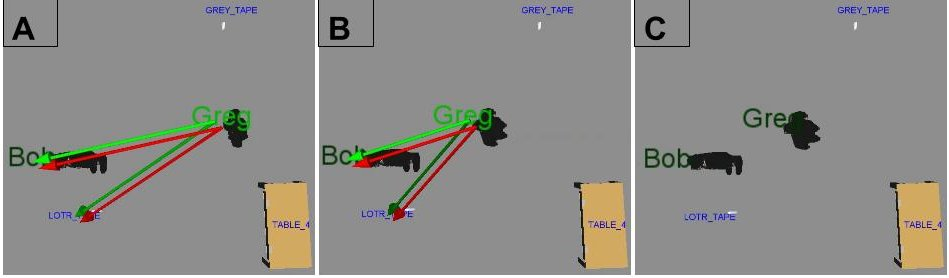
\includegraphics[width=1.0\linewidth]{./img/movingToward.jpg} 
  \caption {Affichage dans rviz des faits liés au module \textit{agent\_monitoring}. La flèche rouge indique ce fait calculé en terme de différentiel de distance alors que la flèche verte indique ce même fait en terme de direction de trajectoire. Sur l'image A et B \textit{Greg} se déplace vers \textit{Bob} ainsi que vers un objet (\textit{LOTR\_TAPE}). Sur l'image A et de façon plus prononcée sur l'image B, les flèches allant vers \textit{LOTR\_TAPE} sont plus sombres, indiquant que la confidence pour ce candidat est moins grande que pour \textit{Bob}. En C Greg s'est arrêté. Les flèches de directions sémantiques ont disparues et le nom de Greg s'est assombri (pour devenir comme celui de Bob qui est immobile).}
  \label{fig:moving}
\end{figure}

Cette visualisation permet de comprendre l'état du monde tel qu'il est perçu par le robot et permet donc de faciliter les explications liées aux agissements du robot, mais aussi de faciliter la configuration d'une nouvelle expérimentation et la recherche d'erreurs lors de l'implémentation de nouvelles fonctionnalités. 

%It uses the position of the entities published by the data gathering component and the areas published by the area manager component as shown in Fig.~\ref{fig:simu} and Fig.~\ref{fig:spencer}. In a future work, we would like to improve this visualization by adding the rendering of other facts, such as the one generated by the agent monitoring component.

Un autre composant déjà évoqué dans la partie \ref{sec:PDG}, permettant de rapidement paramétrer et tester des expérimentations est le module de test \textit{toaster\_simu}. Grâce à ce module, il est possible par une simple requête d'ajouter et positionner des entités dans l'environnement. Il est également possible de contrôler ces entités par une interface clavier. Le module exportera alors en temps réel les données liées à l'état du monde créé par l'utilisateur et ces données seront lues par le module PDG. Il est donc possible, à partir d'un simple script envoyant quelques requêtes, de configurer un environnement d'interaction avec des robots, des humains et des objets. Des scripts python pour configurer un environnement de simulations sont disponibles à titre d'exemple\footnote{https://github.com/Greg8978/toaster-scripts}.


\subsection{Architecture globale}
Les autres modules compris dans l'infrastructure logicielle TOASTER ont une implémentation qui suit les descriptions données précédemment.
Ainsi, le module \textit{area\_manager} permet d'ajouter et de supprimer des zones dans l'environnement à l'aide de requêtes. Le modèle et les raisonnements développés dans ce module suivent la description faite en \ref{sec:zones}. Pour le calcul de l'agencement des différents éléments, un module nommé \textit{SPAR} (pour SPAtial Reasonning) est utilisé. Enfin, pour le suivi des agents décrit en \ref{sec:situationAgents}, le module \textit{agent\_monitoring} a été développé.
Concernant la base de données temporelle, nous avons conçu celle-ci en utilisant la bibliothèque SQLite\footnote{https://www.sqlite.org/}. Ce choix a été fait car cette base de données est très répandue, respecte les conventions SQL et permet une gestion in-memory des données qui augmente les performances en terme de vitesse d'accès à la donnée.

Chacun de ces modules peut être démarré et arrêté à n'importe quel moment de l'interaction. Il peut également recevoir des requêtes ou des messages provenant d'autres composants mais ne dépend pas directement des autres. Par exemple, il est possible d'utiliser le module de raisonnement sur les zones (\textit{area\_manager}) sans \textit{PDG}. Cependant il est nécessaire, si l'on veut que les calculs sur la présence d'entités dans les zones soit effectif, que le module \textit{area\_manager} reçoive les données correspondantes.
De même, la base de données temporelle a été conçue pour pouvoir lire des listes de faits en entrée mais il est possible de paramétrer celle-ci afin de définir quelles listes de faits doivent être lues.
Ceci permet de facilement remplacer un module de l'architecture sans impacter les autres modules, dans la mesure où ce nouveau module respecte les conventions de formats de données d'entrée et sortie.

Pour aider à la compréhension, nous proposons le schéma d'architecture \ref{fig:toasterArch} qui présente comment les données des différents composants peuvent s'interfacer.


\begin{figure}[ht!]
 \centering
  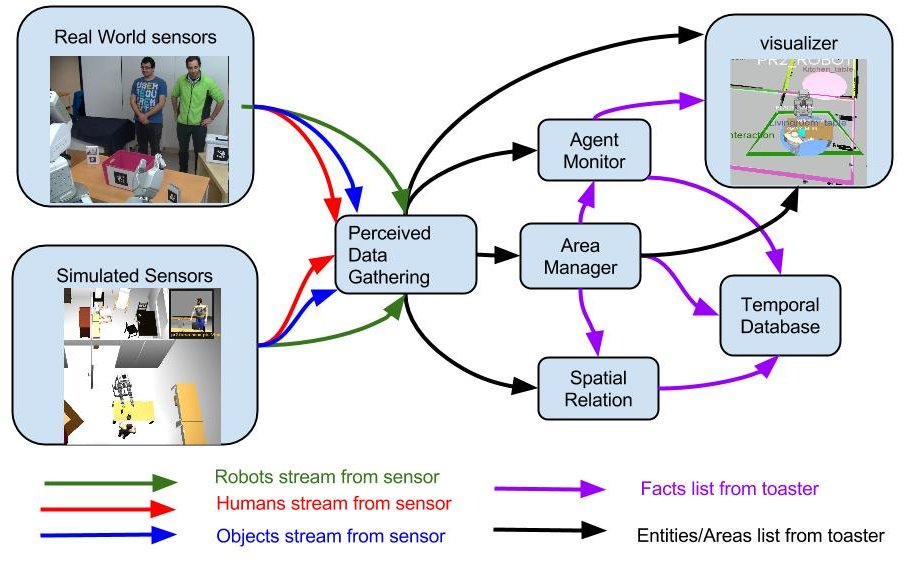
\includegraphics[width=0.99\linewidth]{./img/toasterArch.jpg} 
  \caption {Architecture de l'infrastructure logicielle TOASTER avec les différents flux d'échanges de données}
  \label{fig:toasterArch}
\end{figure}

\section{Résultats expérimentaux}
Pour illustrer l'utilisation possible de TOASTER, nous présentons ici deux expérimentations utilisant l'infrastructure logicielle.

\subsection{Le robot guide}

L'une des premières applications de TOASTER a été de l'utiliser comme composant d'estimation de la situation pour un robot guide adaptatif, proactif et prenant en compte les humains \cite{fioreicsr2015}.

Pour cette application, le robot doit guider un groupe d'utilisateurs à travers une zone de transit (potentiellement bondé), pour les amener à l'endroit choisi.
L'un des défis de ces travaux était de guider les personnes de façon socialement acceptable et en prenant en compte le confort des usagers.
Pour ce faire, le robot adapte sa vitesse au groupe, ce afin de tous les amener à leur destination avec une allure qui satisfasse la plupart des usagers et évite que certains utilisateurs n'abandonnent.

Pour atteindre ces objectifs, nous avons utilisé: (1) le module PDG pour regrouper les données capteurs afin de générer et maintenir le modèle de l'état du monde; (2) les faits générés par le module de gestion des zones (area\_manager); (3) les faits générés par le module de suivi des agents (agent\_monitoring), pour comprendre la situation du groupe. 

Concernant le module de gestion des zones, deux types de zones ont été crées: les zones de guidage et les zones d'activité. Les premières sont liées au robot et évoluent donc avec sa position et son orientation. Elles sont utilisées pour évaluer la configuration des utilisateurs par rapport au robot guide, ce qui lui permet d'adapter sa vitesse en fonction de la configuration du groupe.
L'idée est de créer trois zones de guidage autour du robot pour savoir si la configuration des utilisateurs indique qu'ils souhaitent que le robot aille plus vite ou si l'un d'entre eux a du mal à suivre.
Les trois zones sont appelées \textit{slow}, \textit{following} et \textit{pushing} et sont configurées comme indiqué dans la figure \ref{fig:spencer}.
L'idée est que, (1) si l'un des membres du groupe est dans la zone \textit{slow} (loin du robot) le robot \textit{ralentit}. (2) Si 1) est faux et la majorité du groupe est dans la zone \textit{pushing} (proche ou sur les côtés du robot) le robot \textit{accélère}. (3) Si 1) et 2) sont fausses, signifiant qu'à la fois aucun humain ne se trouve dans la zone \textit{slow} et que la majorité des humains se trouvent dans la zone \textit{following}, le robot \textit{continue} avec la même allure.

Le deuxième type de zones est statique, lié à une position de l'environnement, et déclenche des calculs sur les humains s'y trouvant. Ces calculs concernent les distances, le mouvement et l'orientation par rapport à un point d'intérêt (comme par exemple un écran). En utilisant ces zones, le système peut détecter l'activité humaine (par exemple que l'humain regarde un écran d'information ou l'humain se dirige vers les toilettes). Cette estimation de la situation donne au robot la capacité de détecter quand un ou plusieurs des humains du groupe guidé, est investi dans une activité temporaire. Le robot peut ensuite distinguer entre les situations où il devrait abandonner le guidage de certains usagers de situations où il devrait attendre les humains, voir même les aider de façon pro-active (par exemple proposer des informations s'il détecte qu'un humain regarde un panneau d'informations).

%This situation assessment gives, to the robot, the capacity to detect that one or more of the human followers are involved in a temporary activity. The robot can then disambiguate between situation where it should give up on guiding and situation where it should wait for the humans, or even proactively help the humans involved in the activity.

%TODO: rewrite to adapt to toaster
%To be relevant, reasoning on humans should be linked to the environment. The system is able to create activity areas in the environment and link them to different kind of computations. An activity area is a polygonal or circular area, which can be fixed or linked and updated with an entity's (object, human or robot) position. For now, we studied and experimented different activity areas: a) Information Screen Area, linked to information screens present in the environment; b) Touristic Point Area, linked to interesting attractions in the environment.
%Using these areas, the system can detect human activities (e.g. human is looking at an information screen, human is looking at an attraction).


%
%We believe that to be socially acceptable, the robot should adapt its speed to the group. By setting its own pace at the start of the scenario the robot  would risk of being too slow, annoying the users, or too fast, which would lead the robot to constantly stop to wait for the group, producing an awkward behavior.

%The robot defines a desired range of distance $r$ from the group. The distance of the  members of the group from $r$ will influence its actions. 1) If there is a member of the group farther than $r$ the robot will \textit{decelerate}. The main goal of a guide robot should still be guiding all of the group, and so the robot will give priority to people that would like a slower speed. 2) If 1) is false, and the majority of the group is closer to the robot than $r$, the robot will $accelerate$. 3) If 1) and 2) are false, the robot will continue at its pace.


%In some situation, the robot needs to suspend the task, because the group has stopped following it. In this case, the robot should estimate if this suspension of the collaborative scenario is temporary or permanent, and in the latter case abandon the task. We estimate this information using the Suspend Model and the activity areas from Situation Assessment. We link activity areas to the maximum time we expect that the group will be involved in the linked activity, and with a set of proactive actions that the robot can choose to execute.

%In this paper, we investigated a single possible proactive behavior: giving information. In this case, if we detect that one or more  members
%of the group has stopped following because it is looking at a touristic sight, or at an information screen, the robot can try to engage him and offer related information. At the moment, we just propose a simple routine-based framework for this behavior, and plan to further study it in the future. We believe that the solution of this problem could be rich, and that the robot should estimate the reaction of the group during the execution of its proactive behavior, in order to be able to interrupt if the group doesn't want to be helped or to resume the original task if they are satisfied by the robot's actions.

 \begin{figure}[ht!]
 \centering
 \begin{tabular}{cc}
   \vspace{-5pt}
  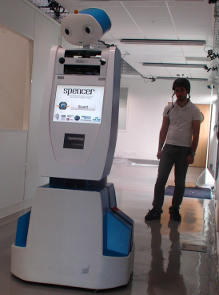
\includegraphics[width=0.4\textwidth]{img/spencer_guidingShrink.png} &
  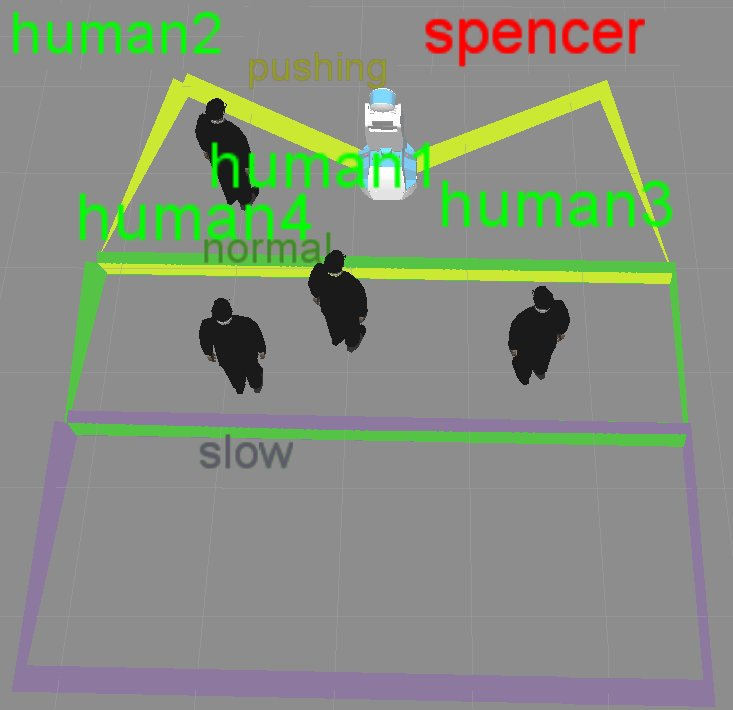
\includegraphics[width=0.56\textwidth]{img/toaster_spencer.jpg}
 \end{tabular}
 \caption{Le robot Spencer, dans le monde réel (à gauche) et dans TOASTER (à droite) avec les zones qui lui sont attachées pour guider les humains.}
 \label{fig:spencer}
  % \vspace{-10pt}
 \end{figure}
 
 
\subsection{Le robot coéquipier}
L'un des autres projets utilisant l'infrastructure logicielle TOASTER visait à construire un robot pour travailler avec un humain sur une chaîne d'assemblage.
Dans ce scénario, le robot partage l'espace de travail avec un humain. Par conséquent, il est essentiel de pouvoir estimer à tout moment la situation spatiale de l'homme et son activité.
Le système se repose sur le module \textit{PDG} de TOASTER pour regrouper les données depuis les capteurs et construire le modèle d'environnement.
Il utilise également le module \textit{SPAR} pour avoir une représentation symbolique de l'état du monde, le module de gestion des zones pour savoir à quelle station de travail l'humain se trouve et le module de suivi des agents pour estimer l'action courante de l'homme.
En utilisant les faits provenant de ces modules, lui procurant une représentation symbolique de l'état du monde et de la situation de l'interaction, le robot est capable d'adapter son comportement à l'humain avec lequel il collabore.
La première façon d'utiliser les informations de TOASTER est d'assurer la sécurité en arrêtant le déplacement du robot lorsque l'homme est dans la même zone de travail et lorsqu'il est en train de se déplacer.
Un autre moyen de s'adapter est de transmettre la représentation symbolique  de l'état du monde (l'ensemble des faits) à un planificateur afin d'aider l'homme de façon proactive. En effet, avec la connaissance de l'état du monde actuel, reliée à la compréhension de l'activité de l'homme, le robot peut estimer l'étape actuelle du plan à accomplir et agir afin d'aider l'homme pour les étapes suivantes du plan. Par exemple, lorsque l'homme est en train de nettoyer une pièce à assembler, si l'étape suivante est de visser cette pièce, le robot peut apporter la visseuse à l'homme. L'image \ref{fig:saphari} illustre la situation où le robot détecte que l'homme tend le bras et est orienté en direction du robot. En utilisant ces faits, le robot suppose que l'homme est prêt à recevoir l'objet et le lui donne.

%Add TOASTER image?

 \begin{figure}[ht!]

 \centering
 \begin{tabular}{cc}
  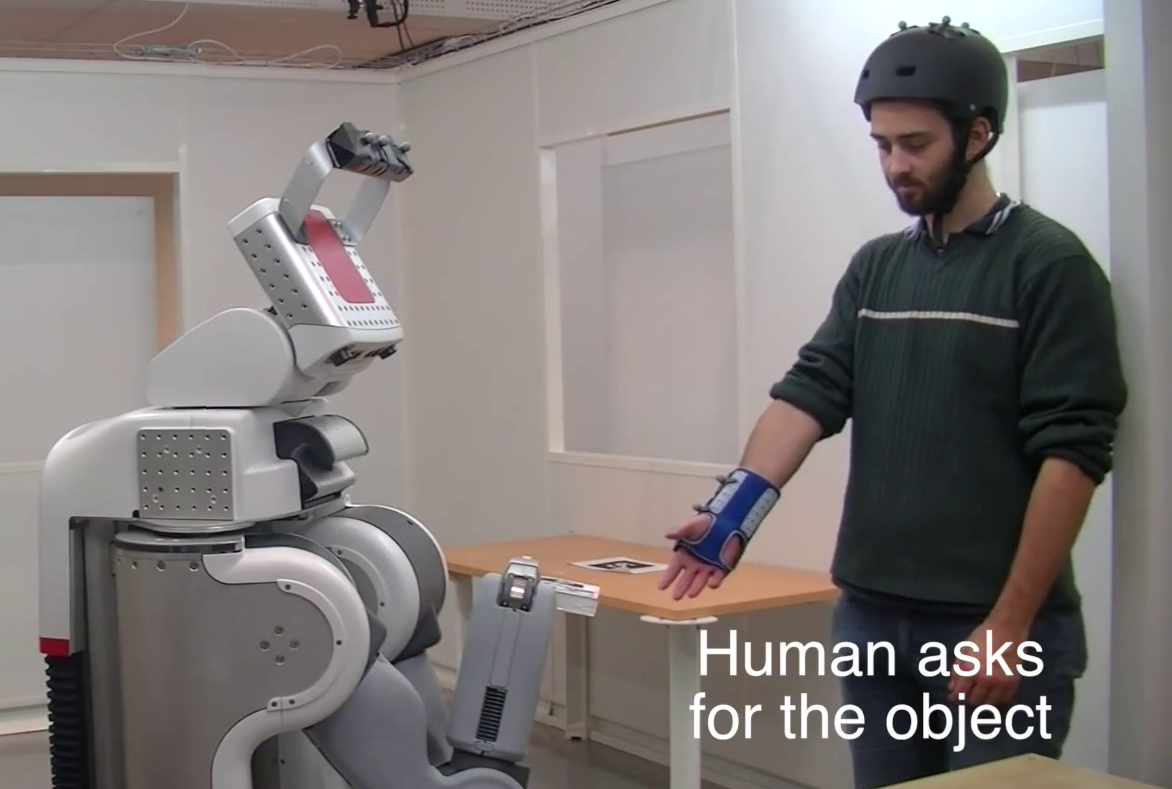
\includegraphics[width=0.7\textwidth]{img/sapharishrink.png}
 \end{tabular}
 \caption{Le robot détecte que l'homme demande l'objet en utilisant la posture de l'homme reconnue par le module de suivi d'agent de TOASTER. Ici, un système de capture de mouvement est utilisé pour suivre les positions de la tête et du bras de l'homme.}
 \label{fig:saphari}
  \vspace{-15pt}
 \end{figure}
 
 
 Ces deux exemples d'utilisation de l'infrastructure logicielle dans deux projets différents illustrent la généricité, la simplicité de reconfiguration grâce à l'architecture modulaire, ainsi que la polyvalence de TOASTER. Dans ces deux projets d'interaction homme robot, les faits générés par TOASTER ont permis de fournir les informations nécessaires à la couche décisionnelle pour pouvoir s'adapter à l'homme et donner un comportement socialement acceptable au robot.

%\section{Gestion de l'Incertitude}
%TODO?
%humain prends un objet dans panier à 2 objets
%-> 50 / 50?
% 
%\section{Bilan}



\ifdefined\included
\else
\bibliographystyle{acm}
\bibliography{bibliorachid}
\end{document}
\fi
